\chapter{Local Stability Analysis}
\label{ch:06} 

\chaptermark{Chapter 6}

\abstract{This chapter introduces the key concepts and methods involved in performing a stability analysis of steady states for nonlinear dynamical systems. Steady states, or fixed points, are defined as constant solutions to a differential equation that do not change over time. Their stability determines whether nearby solutions will converge or diverge from the steady state. While graphical analysis can assess stability in 1D, a more rigorous analytical approach is required for higher dimensions. The method developed is to linearize the nonlinear dynamics near a steady state, resulting in a linear approximation governing small perturbations from the fixed point. The stability criterion is then derived from the solution to this linearized system---a steady state will be stable only if perturbations decay over time, indicated by the slope of the original function being negative at that point. This technique allows classification of steady state stability across any system dimensionality using analytical mathematics.}

\vspace{1cm}

\section{Introduction}

In the preceding chapters, we introduced basic linear population dynamics models and analyzed how their behavior evolves over time. However, more realistic representations often involve nonlinear differential equations. Attaining a rigorous global understanding of these models necessitates a formal stability analysis of their steady states. A steady state corresponds to a constant solution. For a population, this represents an equilibrium point at which birth and death rates precisely balance. Studying the stability of steady states allows for the classification of long-term dynamical behavior and the discernment of global dynamics arising from local perturbations.

Just as a balance at rest indicates equilibrium but imparts no insight into subsequent motion upon disturbance, steady states alone do not reveal dynamical fate. Their stability determines their attracting or repelling character, with implications for qualitative trajectories that may resemble balls inducted into concavities or convexities. Linearizing functions near steady states permits estimation of the evolution of small deviations, providing local qualitative forecasts. When stability analysis and linearization are combined, they provide qualitative understanding that exceeds model solutions, just as one may predict a ball's motion from terrain alone despite transients obscuring endpoints. This chapter will introduce the tools to perform local stability analysis of 1-dimensional dynamical models.

\section{Steady States}

Consider the univariate ordinary differential equation:
\begin{equation}
\frac{dx}{dt} = f(x),
\label{eq:06.01}
\end{equation}
wherein $f(x)$ denotes an arbitrary smooth function. Steady states, or fixed points, for this differential equation represent unchanging constant solutions independent of time ($t$).

Let $x(t) = x^*$ represent a steady state. Its derivative with respect to time is null given its lack of time-dependence. Furthermore, by definition it must satisfy Eq. \eqref{eq:06.01}. Upon substitution, we obtain:
\begin{equation*}
f(x) = 0
\end{equation*}
Accordingly, the steady states equate to the roots of function $f(x)$. This provides a method for determining the fixed points of any first-order ordinary differential equation by resolving the relationship $f(x^*)=0$.

\section{Assessment of Fixed Point Stability via Graphical Analysis}

Consider the function $f(x)$ depicted in Fig. \ref{fig:06.01}. Two roots, denoted $x_1$ and $x_2$, of the equation $f(x)=0$ are evident. Consequently, these locations define the steady states of the differential equation $dx/dt=f(x)$.

\begin{figure}
    \centering
    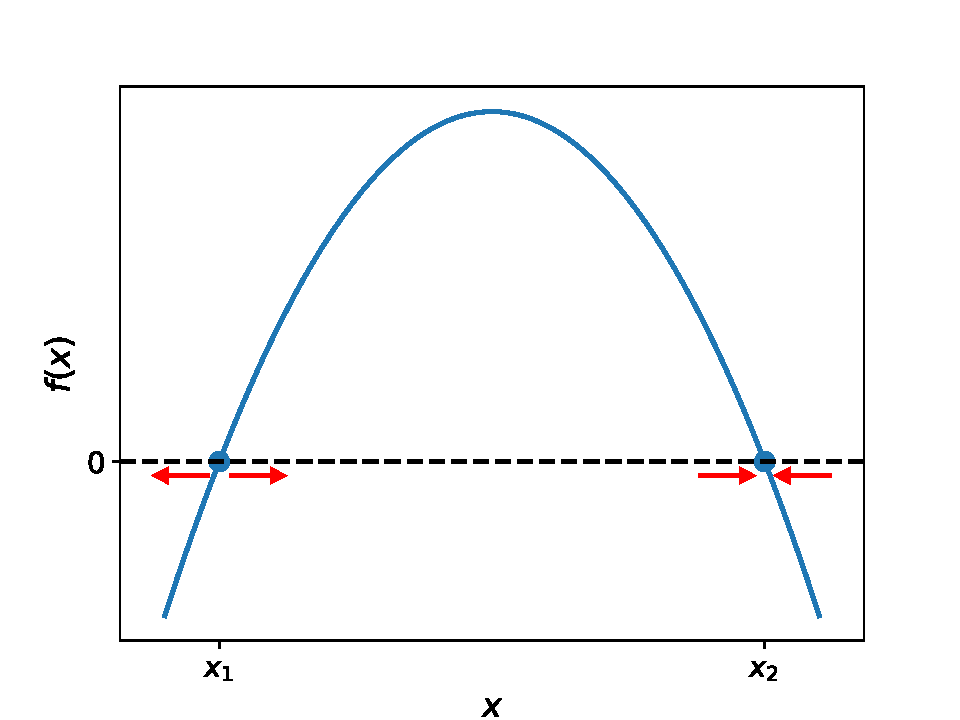
\includegraphics[width=3in]{Figures/fig-06.01.pdf}
    \caption{Graphical depiction of the function $f(x)$ with two roots. This figure illustrates the function $f(x)$ which possesses two roots, denoted by $x_1$ and $x_2$. The slope of $f(x)$ is positive in the vicinity of $x_1$, as depicted by the upward sloping tangent. In contrast, the slope is negative near $x_2$, as shown by the downward sloping tangent. These slope characteristics determine the qualitative behavior of solutions initialized proximate to the steady states. Specifically, red arrows indicate that perturbations tend to diverge from $x_1$ while converging towards $x_2$. Therefore, $x_1$ represents an unstable fixed point whereas $x_2$ denotes a stable steady state. This graphical analysis conveys how the slope's sign at steady state locations qualifies their attracting or repelling nature.}
    \label{fig:06.01}
\end{figure}

Let us now analyze the stability of the fixed points. Consider $x_1$ and note the positive slope of $f(x)$ at this location. A positive slope implies that for any initial condition marginally greater than $x_1$, the value of $f(x)$ will be positive. Accordingly, this yields a positive rate of change for the value of $x$. Thus, the solution will move in a progressively greater direction, distancing itself from $x_1$. Similarly, for any initial value slightly less than $x_1$, the slope is such that the rate of change of $x$ is negative. Consequently, the solution will decrease over time, drifting ever farther from $x_1$. From this analysis, we can see that $x_1$ is unstable as it repels nearby solutions over time.

In contrast, let us examine the stability of the other fixed point, $x_2$. At this location, the slope of $f(x)$ is negative. Therefore, for any initial condition marginally greater than $x_2$, the value of $f(x)$ will be negative. This implies the rate of change of $x$ will also be negative, causing the solution to decrease in value over time and move closer to $x_2$. Similarly, for initial values slightly less than $x_2$, the negative slope indicates the rate of change of $x$ is positive. Hence, the solution will increment in value, again tending towards $x_2$. We can thus deduce that perturbations from $x_2$ will be attracted back to this fixed point location over time. Consequently, $x_2$ is stable as it attracts solutions.

In summary, this graphical analysis demonstrates that the stability of a fixed point for the differential equation $dx/dt=f(x)$ is determined solely by the sign of the slope of the function $f(x)$ evaluated at that fixed point. A positive slope implies perturbations will move further away from the fixed point over time, characterizing it as unstable. In contrast, a negative slope signifies that perturbations will be attracted back to the fixed point location, marking it as stable.

\section{Local Stability Analysis}

While the preceding graphical approach provides useful qualitative insights into fixed point stability for univariate systems, it cannot not be readily generalized to higher dimensions. The graphic analysis relies on visualizing the slope of a scalar-valued function, which is only possible for one-dimensional models. However, real-world phenomena often evolve according to multidimensional dynamical systems that cannot be embedded in two-dimensional space for intuitive slope evaluation. Therefore, a more systematic technique is required that permits stability classification of fixed points for differential equations inhabiting abstract dimensionalities. In this section, we develop the method of local stability analysis through linearization. By approximating nonlinear dynamics near steady states via linear functions, this approach furnishes a quantitative framework to assess stability in any dimensional system. These analytical tools supersede qualitative geometric intuitions, instead providing mathematics directly applicable to complexity beyond what may be visualized. 

Consider once more the differential equation:
\begin{equation}
\frac{dx}{dt} = f(x).
    \label{eq:06.02}
\end{equation}
We want to analyze the stability of a steady state value $x^*$. To do this, we look at an arbitrary solution $x(t)$ that starts out close to $x^*$. For the steady state to be locally stable, we need to show that $x(t)$ converges to $x^*$ as time goes to infinity:
\begin{equation}
\lim_{t\to\infty} x(t) = x^*
    \label{eq:06.03}
\end{equation}

It's helpful to define the ``distance function" $\delta x(t)$:
\begin{equation}
\delta x(t) = x(t) - x^*.
    \label{eq:06.04}
\end{equation}
This tells us how far $x(t)$ is from the steady state $x^*$ at any time $t$. For our analysis to work, $\delta x(t)$ needs to stay much smaller than $x^*$ as time passes.

We can write the stability condition in terms of $\delta x(t)$ as well:
\begin{equation}
\lim_{t\to\infty} \delta x(t) = 0.
    \label{eq:06.05}
\end{equation}
In other words, for $x^*$ to be stable, any small perturbations need to disappear over long times.

We seek to derive the governing differential equation for the dynamics of $\delta x(t)$. It can be readily shown from its definition in Eq. \eqref{eq:06.04} that:
\begin{equation*}
\frac{d\delta x(t)}{dt} = \frac{dx(t)}{dt}.
\end{equation*}
Substituting this expression and Eq. \eqref{eq:06.04} into the original system dynamics in Eq. \eqref{eq:06.02} yields:
\begin{equation*}
\frac{d\delta x}{dt} = f(x^* + \delta x).
\end{equation*}
Leveraging the assumption that $\delta x$ is small relative to $x^*$, we can approximate $f(x^* + \delta x)$ via a Taylor series expansion truncated after the first order term:
\begin{equation*}
f(x^* + \delta x) \approx f(x^*) + f'(x^*)\delta x,
\end{equation*}
where $f'(x^*)=d f/d x|_{x=x^*}$. Furthermore, since $x^*$ defines a steady state, $f(x^*)=0$. Thus, the differential equation for $\delta x$ reduces to the following linear form:
\begin{equation*}
\frac{d\delta x}{dt} = f'(x^*)\delta x.
\end{equation*}
The solution to this equation takes the form
\begin{equation*}
    \delta x(t) = \delta x_0 e^{f'(x^*) t},
\end{equation*}
where $\delta x_0$ denotes the initial perturbation from the steady state $x^*$. It is evident from this last equation that a necessary condition for $\delta x(t)$ to asymptotically approach zero as $t\to\infty$ is that $f'(x^*)<0$. In other words, the steady state $x^*$ will only exhibit stable behavior if the slope of the function $f(x)$ is negative when evaluated at $x=x^*$. In summary, local stability is assured only if perturbations decay over time, which occurs solely when the linearized dynamics represented by $f'(x^*)$ are negative. 

\section{Discussion}

In this chapter, we introduced the method of local stability analysis and applied it to determine the stability of steady states for a univariate nonlinear dynamical system. Through linearization near steady states and solution of the resulting linear differential equation governing perturbations, we recovered the same criterion for stability established by the graphical analysis in the previous chapter---namely, that stability is ensured only when the slope of the governing function is negative, as evaluated at the steady state. Interestingly, this analysis arrived at the same qualitative conclusion through an analytical approach, rather than a geometric visualization. This mathematical technique has the advantage of being readily generalized to higher-dimensional systems that cannot be depicted graphically. The method of local stability analysis through linearization provides a systematic framework to assess fixed point stability for nonlinear dynamical models of any dimensionality. In this way, insights into long-term dynamical behavior near steady states can be captured quantitatively rather than relying on low-dimensional intuitions. This analytical approach will prove invaluable for nonlinear multi-species population and ecosystem models in subsequent chapters.

\section*{Exercises}

Find the steady states and characterize their stability for the following one-dimensional differential equations:
\begin{enumerate}
    \item $\displaystyle \frac{dx}{dt} = 2 x - 6$. \vspace{2mm}
    \item $\displaystyle \frac{dx}{dt} = x^2 - 4$. \vspace{2mm}
    \item $\displaystyle \frac{dx}{dt} = (x - 2)^2$. \vspace{2mm}
    \item $\displaystyle \frac{dx}{dt} = -x^3 + 2x$.
\end{enumerate}